\section{Anomaly Detection}
\label{back:anomdet}

\textit{Anomaly detection} is about identifying observations that can be deemed inconsistent with the rest of the dataset \cite{anomaly}. These anomalies can also be called outliers, surprises, or exceptions, depending on the domain. Anomaly detection can be used on all kinds of data, from images to time series. There are three main types of anomalies: \textit{point anomalies}, \textit{contextual anomalies}, and \textit{collective anomalies}.

While point anomalies target single instances that differ from the rest of the dataset, collective anomalies target groups of instances that together form an anomaly. Contextual ones, as in the word, require context to determine whether or not an anomaly has been detected and is typically found in time-series data.

%Anomaly detection can be performed in a lot of different ways. From common machine learning tasks such as K-means clustering \cite{7507933}, \Gls{svm} \cite{10.1007/978-3-540-28647-9_97}

%\begin{figure}[!h]
%    \centering
%    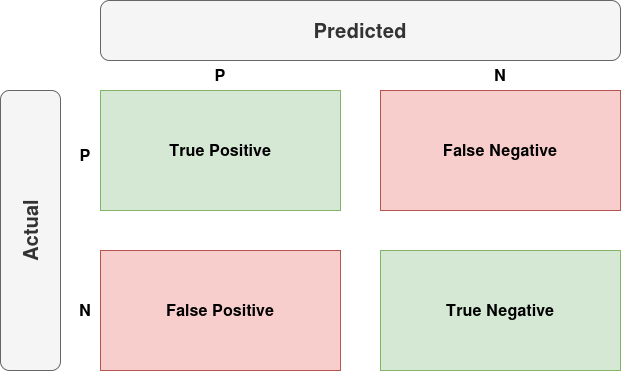
\includegraphics[width=0.5\linewidth]{figures/confmat.png}
%    \caption{Confusion Matrix}
%    \label{fig:confmat}
%\end{figure}

\subsection{Autoencoder-based Anomaly Detection}

Autoencoders are commonly used models for anomaly detection \cite{an2015variational, zhou2017anomaly}. Compared to other models such as \acrfull{pca} \cite{wold1987principal}, autoencoders have been found ''to detect subtle anomalies which linear PCA fails''\cite{sakurada2014anomaly}. By training an autoencoder to reconstruct normal data, any input of anomalous data would yield a higher reconstruction error. If we can find a threshold, we can effectively mark the data as anomalous. 

\begin{algorithm}[!h]
\caption{Autoencoder-based Anomaly Detection}
\label{alg:ad}
\begin{algorithmic}[1]
\small
\Require Normal Data $X$, Anomalous Data $\{x^{(i)} : i = 1, \ldots, N\}$, Threshold $\epsilon$
\Ensure Anomalies $A$
\State $A \gets \emptyset$
\State $D_\phi, E_\theta \gets \text{Train autoencoder on } X$
\For{each $x_i$ in $\{x^{(i)}\}$}
    \State $\text{reconstruction\_error} \gets \|x_i - D_\phi(E_\theta(x_i))\|$
    \If{$\text{reconstruction\_error} > \epsilon$}
        \State $A \gets A \cup \{x_i\}$
    \EndIf
\EndFor
\State \Return $A$
\end{algorithmic}
\end{algorithm}

In Algorithm \ref{alg:ad}, the reconstruction error is calculated using the \acrshort{mae} loss. However, other common loss functions such as \acrshort{mse} can also be used. The important aspect of this approach lies in determining an optimal threshold $\epsilon$. This threshold should be carefully chosen to maximize the amount of correctly identified anomalies and normal data (TP and TN) while minimizing missed anomalies (FN) or incorrectly flagging normal instances as anomalous (FP).


\subsubsection{Anomalies in Time Series}

Time series data from diverse domains, including \acrshort{das}, offer opportunities for anomaly detection. These datasets often contain subtle patterns and contextual anomalies that traditional statistical methods might overlook. Neural networks, particularly those designed for sequential data processing, have emerged as powerful tools for identifying such anomalies. Architectures like \acrfull{lstm} \cite{lstm} and \acrfull{rnn} \cite{medsker2001recurrent} are especially suited for this task \cite{wang2024deep, wei2022lstmautoencoder}. Their built-in memory mechanisms allow them to capture long-range dependencies and temporal context, which is crucial for understanding normal patterns in time series data. Training these networks on typical time series behavior can effectively flag deviations that may indicate anomalies. 

\begin{figure}[!h]
    \centering
    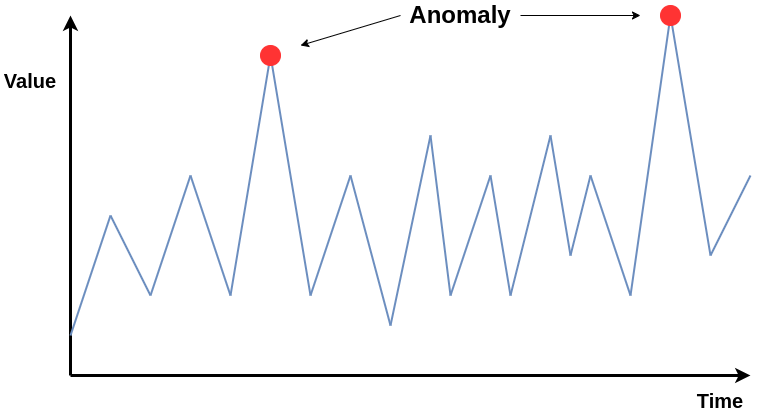
\includegraphics[scale=0.4]{figures/anolay_line.png}
    \caption{Example of anomalies in a time series}
    \label{fig:anomaly_example}
\end{figure}


\subsubsection{Anomalies in images}

Anomaly detection can also be applied to images \cite{beggel2020robust}. In the context of \acrshort{das} data, the data matrix can be viewed as a one-channel image, where the time-domain and frequency-domain can be studied. Architectures like \acrshort{cnn} are especially suited for this task due to their enhanced feature extraction capabilities, as discussed in section \ref{back:cnn}.


